\chapter{Gamma spectrum software analysis}
As was mentioned before in section \ref{char}, the measured gamma spectrum contains many unwanted artifacts like noise, Compton continuum and edges and additional peaks created by various interactions. To properly obtain the count rates on defined energies, the only way is to perform a numerical analysis of measured data. Locations of energy peaks are to be found for example by their characteristic second derivatives. Absolute count rates are then obtained by Gaussian fitting.


\section{Peak searching procedure}
\label{search}
Many commercial programs use peak searching procedures based on algorithm originally developed by M.A. Mariscotti \cite{MARISCOTTI1967309}. This method is based on the numerical second difference assuming that the background can be approximated only by linear functions and thus it vanishes in case of the second derivative. The second fact is that the searched peaks are Gaussians with their specific second derivatives and thus their positions can be found in local minimums (Gaussians have negative second derivatives since their are concave functions). To reduce noise, the second difference is averaged by defined number of steps.
\par
To determine if the found minimum should be considered as peak position (not as a Compton edge etc.), standard deviation and other additional rules based on number of points in specified intervals can be employed. However, algorithm needs input parameters, which are based on raw estimation of FWHM of searched peaks.
\par
For the analysis of measured gamma spectra, this algorithm was implemented in C++ and used to find full energy peaks and other additional peaks as well. The following figures show the example of measured spectra and its second difference plotted along with its standard deviation. The possible candidates onto peak positions can be observed.
\par


\begin{figure}[H]
 \centering
 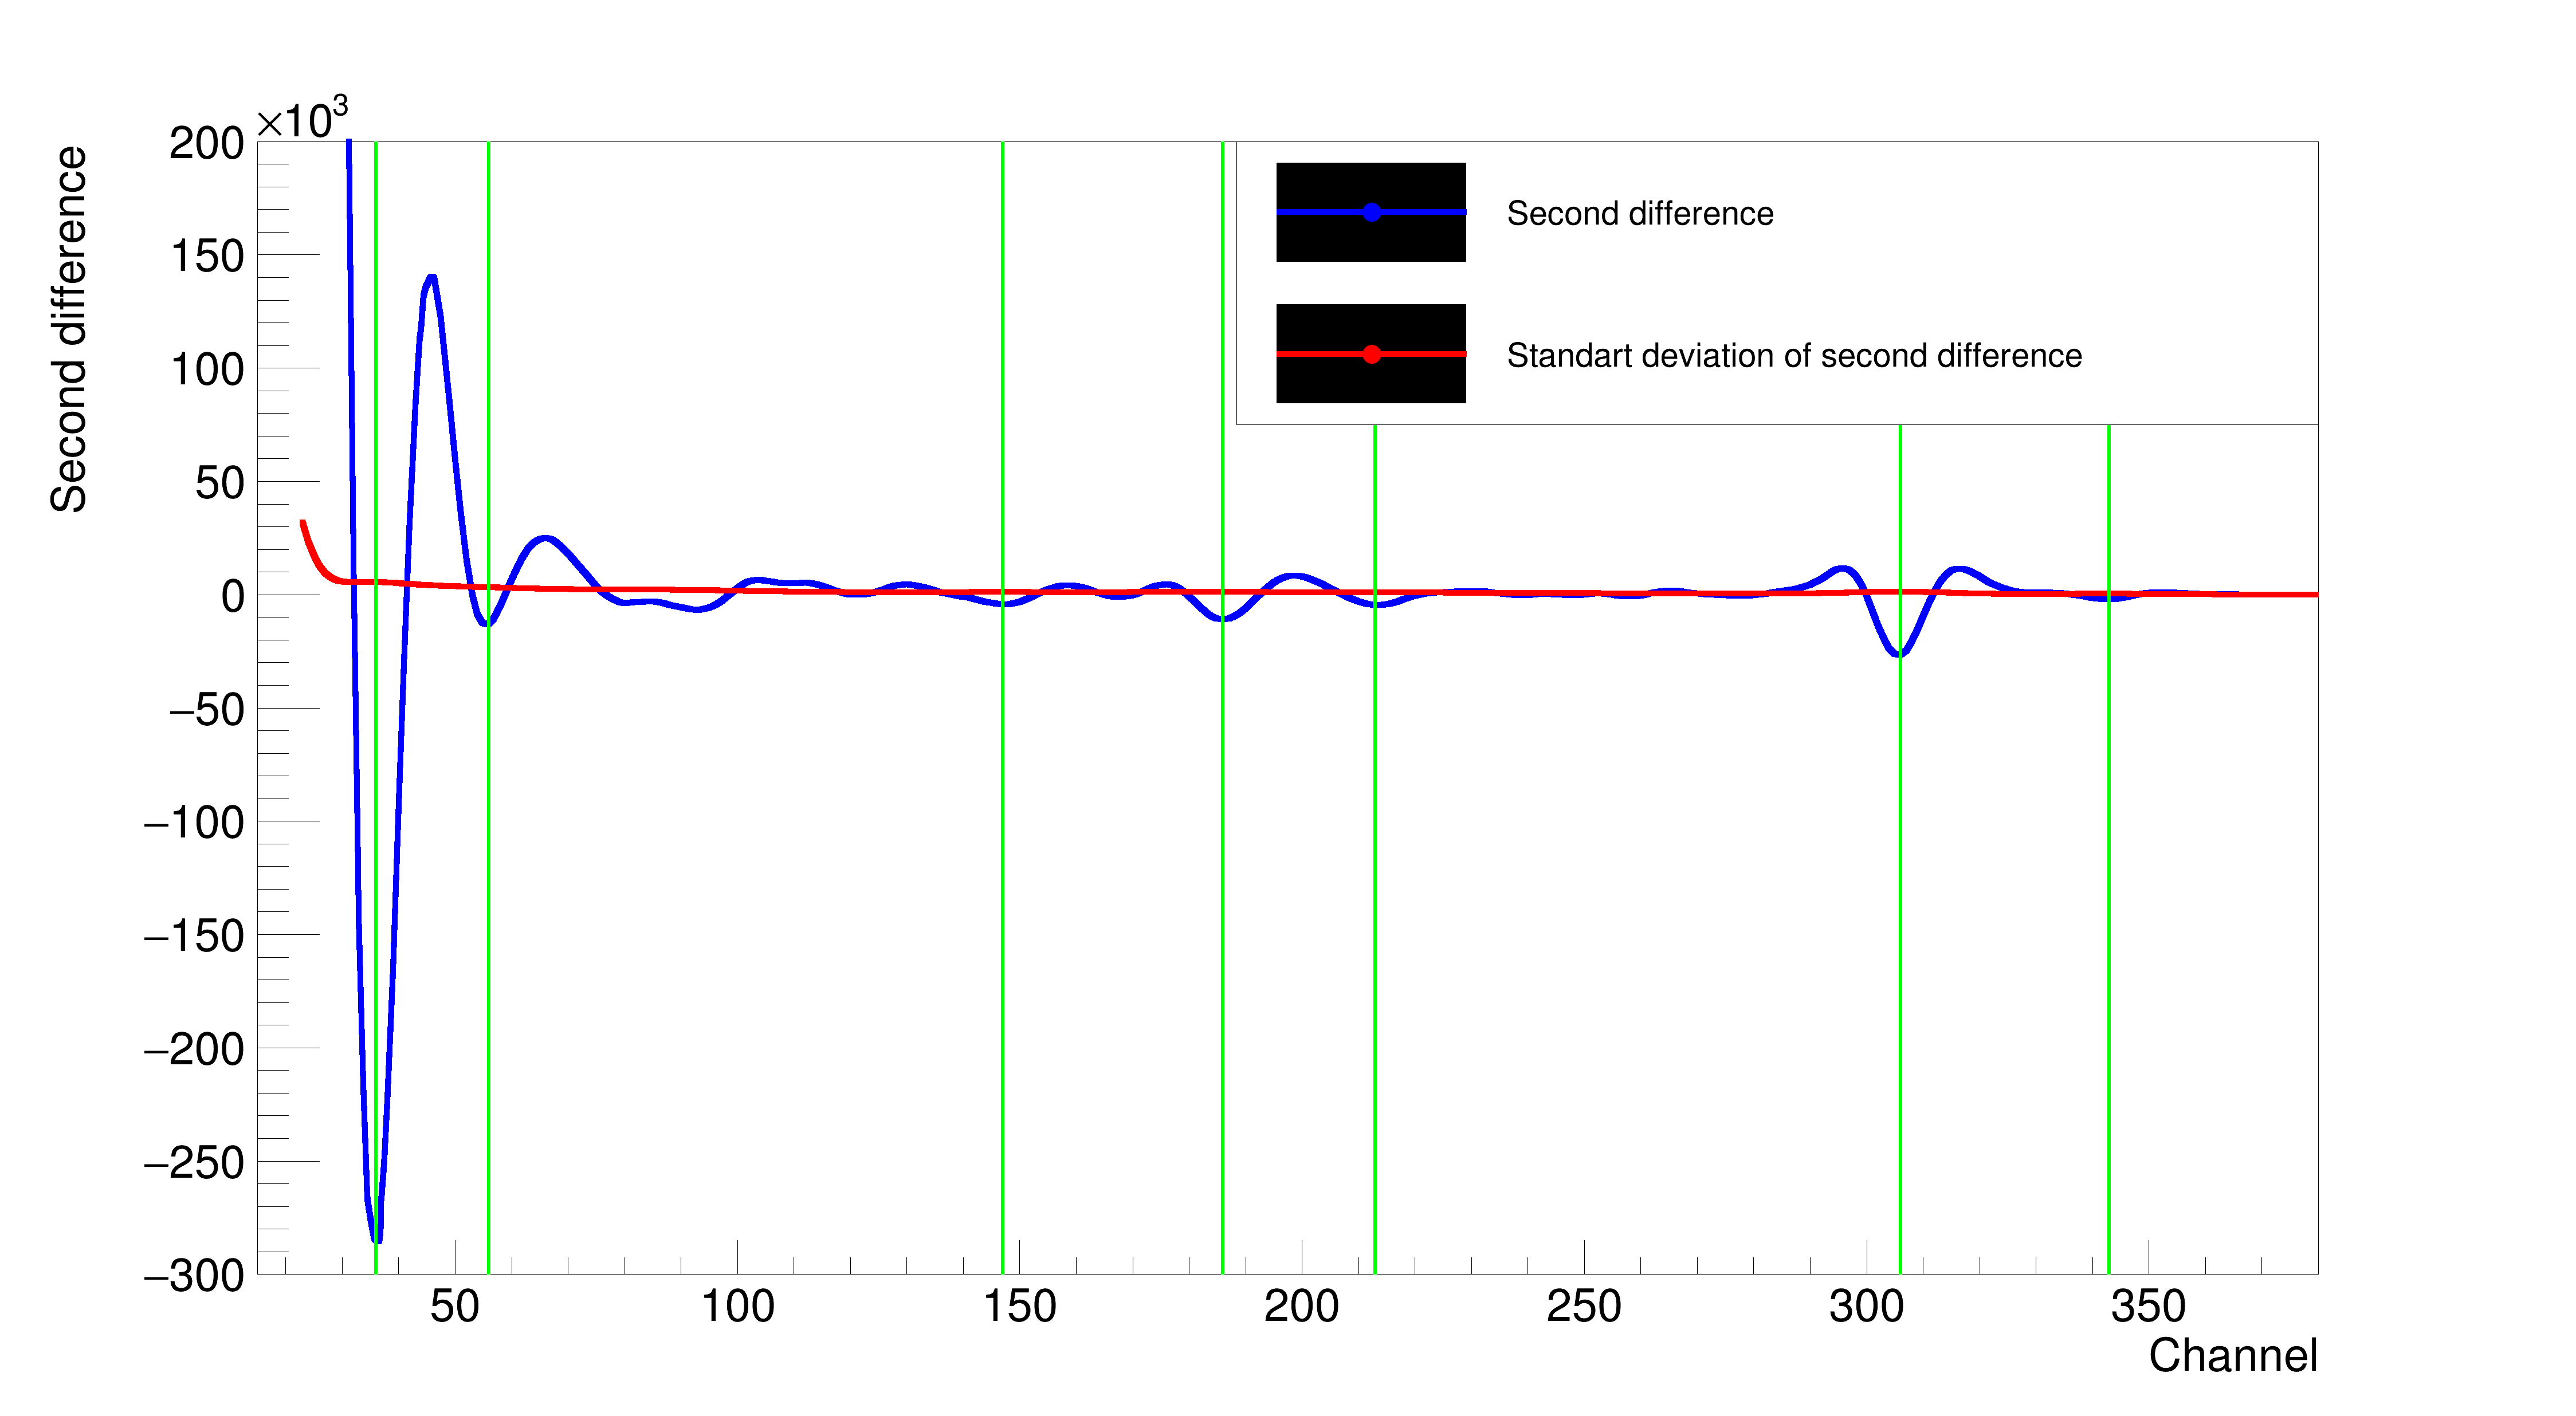
\includegraphics[scale=0.105, angle = 0]{./pictures/SecondDerivGraph.png}
 \caption{Second difference of example spectra along with its standard deviation showing possible candidates (green lines).}
 \label{secondDerivative}
 
\end{figure}

\begin{figure}[H]
 \centering
 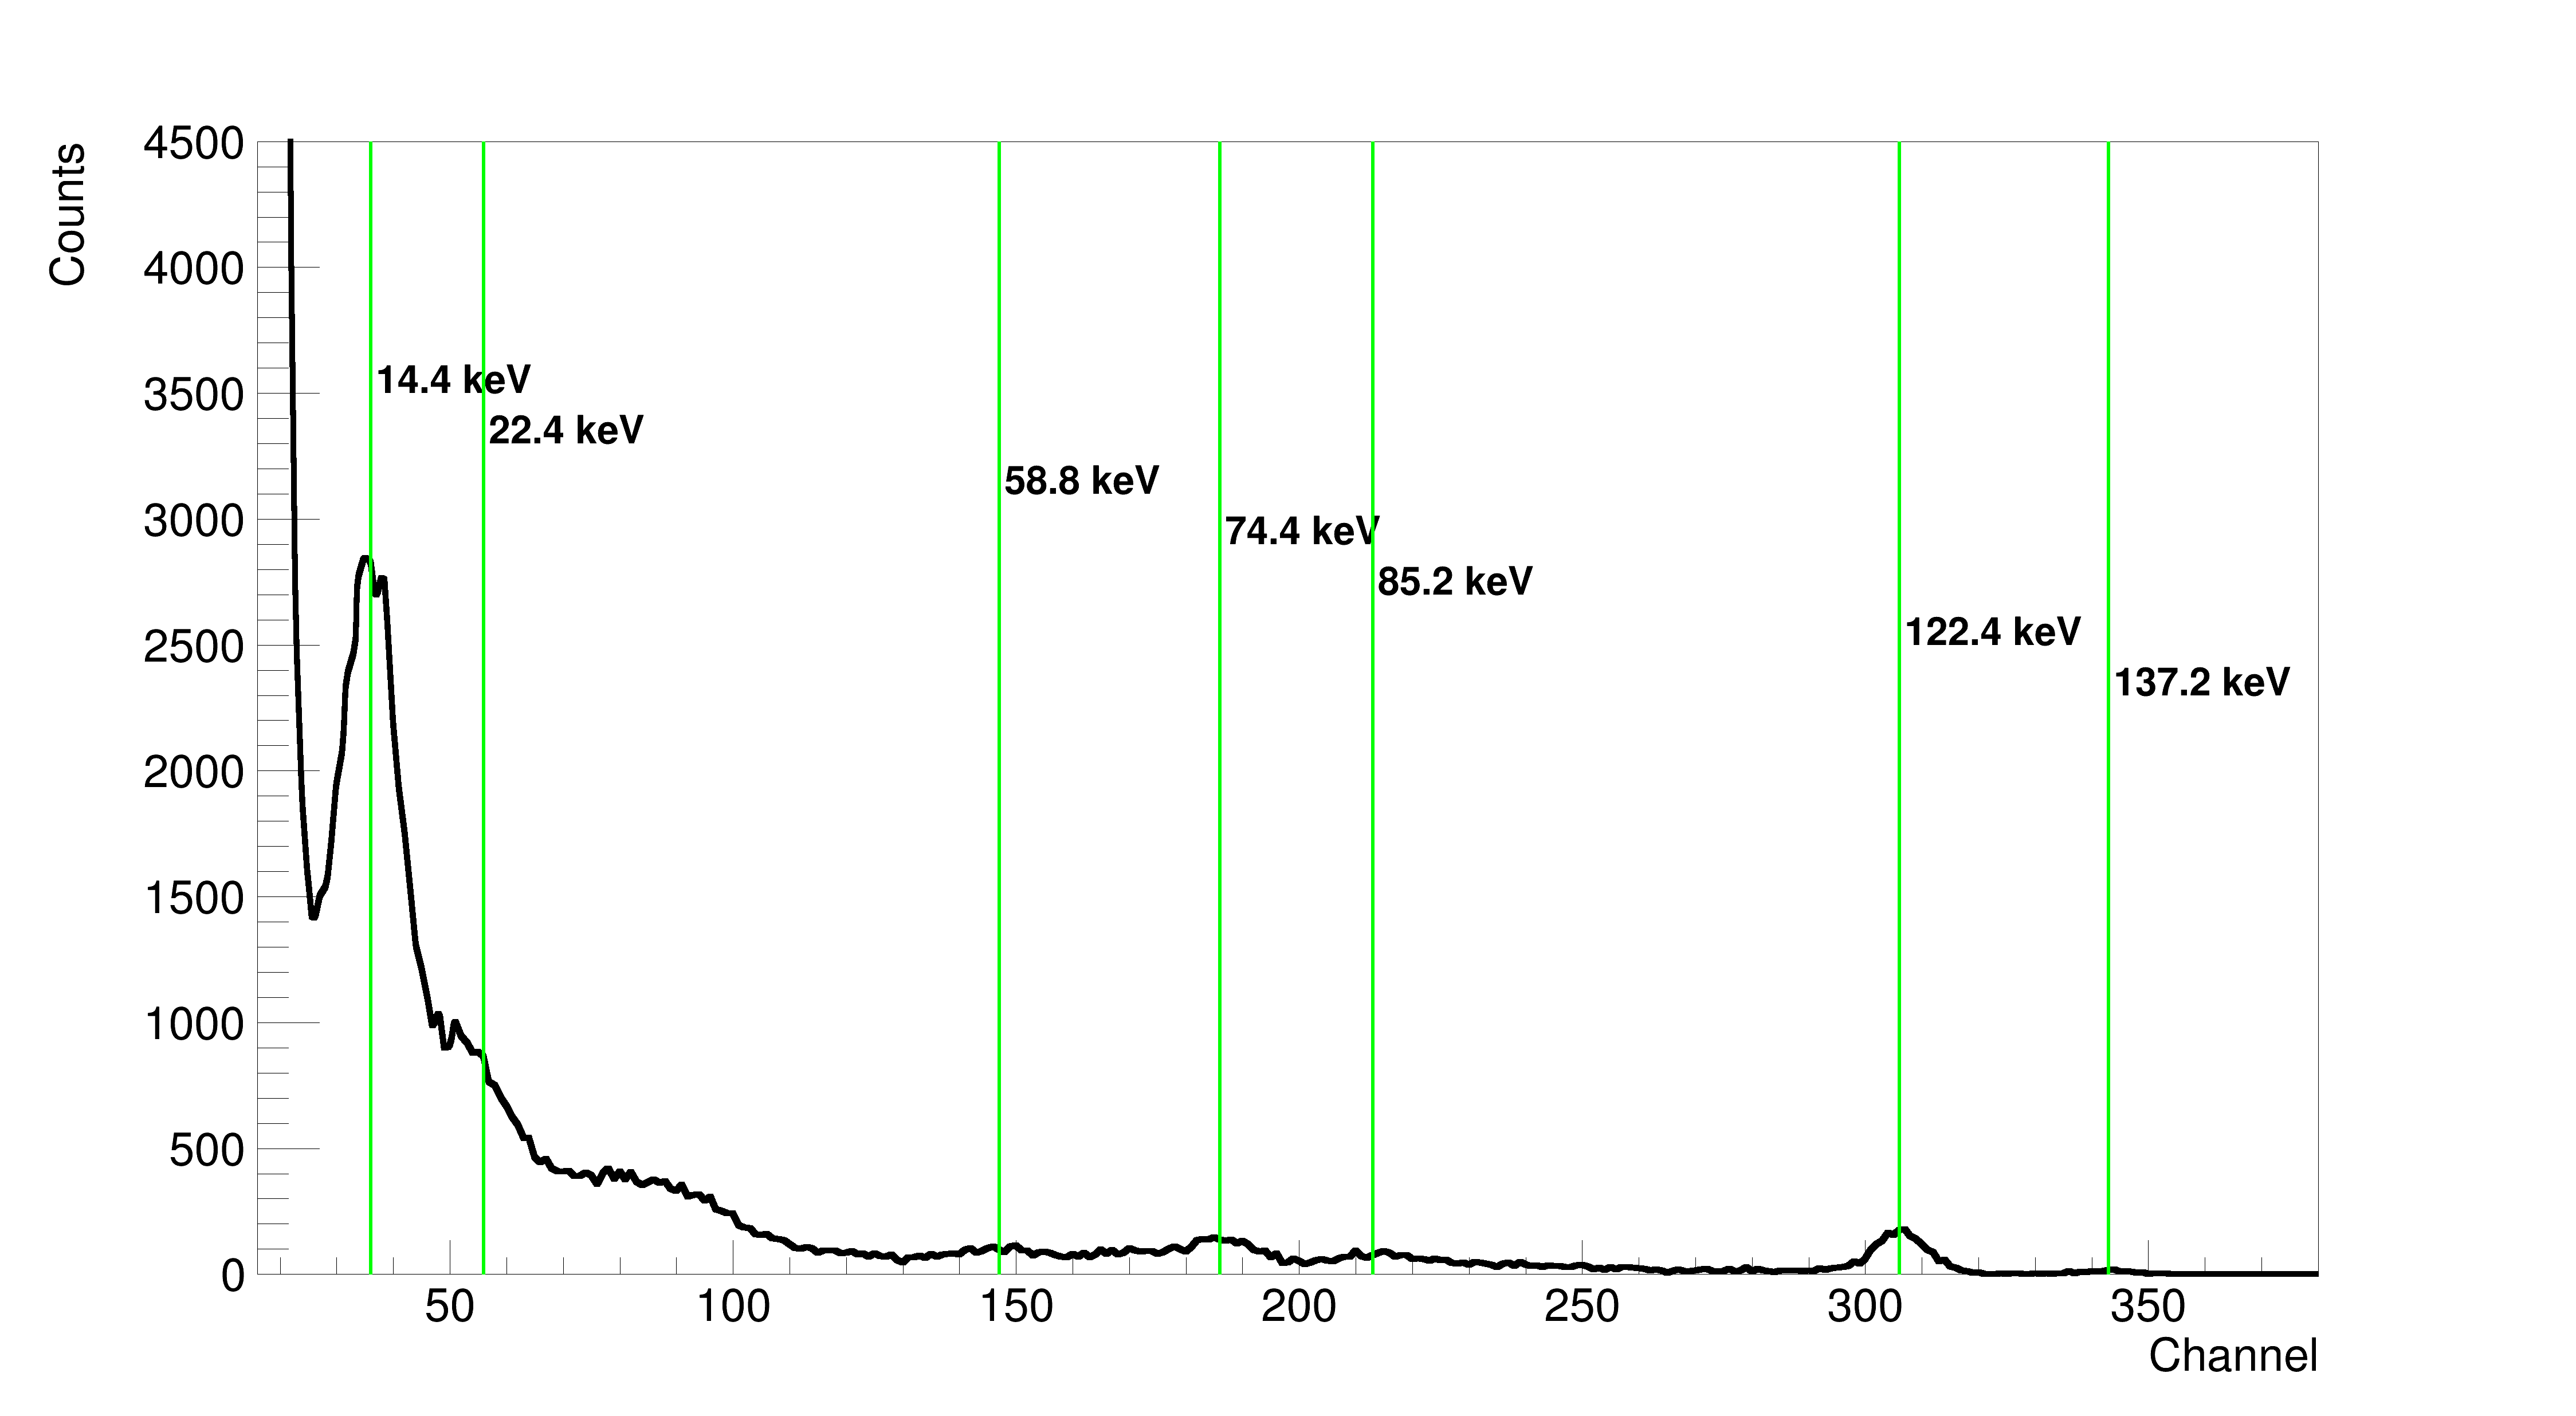
\includegraphics[scale=0.105, angle = 0]{./pictures/DataGraph.png}
 \caption{Example of measured gamma spectra. Green lines mark the energy peaks found by algorithm.}
 \label{Example}
 
\end{figure}
